% **************************************************
% Document Class Definition
% **************************************************
\documentclass[%
	paper=A4,					% paper size --> A4 is default in Germany
	twoside=true,				% onesite or twoside printing
	openright,					% doublepage cleaning ends up right side
	parskip=full,				% spacing value / method for paragraphs
	chapterprefix=true,			% prefix for chapter marks
	11pt,						% font size
	headings=normal,			% size of headings
	bibliography=totoc,			% include bib in toc
	listof=totoc,				% include listof entries in toc
	titlepage=on,				% own page for each title page
	captions=tableabove,		% display table captions above the float env
	draft=false,				% value for draft version
]{scrreprt}%

% **************************************************
% Debug LaTeX Information
% **************************************************
%\listfiles

% **************************************************
% Information and Commands for Reuse
% **************************************************
\newcommand{\thesisTitle}{Bachelorarbeit}
\newcommand{\thesisName}{Philipp Scholz}
\newcommand{\thesisSubject}{NLP-Plattform: Integration und Evaluation von POS-Tagging-Algorithmen}
\newcommand{\thesisDate}{23.April  2019}
\newcommand{\thesisVersion}{Draft}

\newcommand{\thesisFirstReviewer}{Dr. Lars Ackermann}
\newcommand{\thesisFirstReviewerUniversity}{\protect{Universit{\"a}t Bayreuth}}
\newcommand{\thesisFirstReviewerDepartment}{Fakult{\"a}t Mathematik, Physik, Informatik}

\newcommand{\thesisSecondReviewer}{Prof. Dr.-Ing. Stefan Jablonski}
\newcommand{\thesisSecondReviewerUniversity}{\protect{Universit{\"a}t Bayreuth}}
\newcommand{\thesisSecondReviewerDepartment}{Fakult{\"a}t Mathematik, Physik, Informatik}

\newcommand{\thesisFirstSupervisor}{Lars Ackermann}
\newcommand{\thesisSecondSupervisor}{Stefan Jablonski}

\newcommand{\thesisUniversity}{\protect{Universit{\"a}t Bayreuth}}
\newcommand{\thesisUniversityDepartment}{Fakult{\"a}t Mathematik, Physik, Informatik}
\newcommand{\thesisUniversityInstitute}{Institut f{\"u}r Informatik}
\newcommand{\thesisUniversityGroup}{Lehrstuhl f{\"u}r Angewandte Informatik IV}
\newcommand{\thesisUniversityCity}{Bayreuth}
\newcommand{\thesisUniversityStreetAddress}{Universit{\"a}tsstrasse 30}
\newcommand{\thesisUniversityPostalCode}{95447}

% **************************************************
% Load and Configure Packages
% **************************************************
\usepackage[utf8]{inputenc}		% defines file's character encoding
\usepackage[ngerman]{babel} % babel system, adjust the language of the content
\usepackage[					% clean thesis style
	figuresep=colon,%
	sansserif=false,%
	hangfigurecaption=false,%
	hangsection=true,%
	hangsubsection=true,%
	colorize=full,%
	colortheme=bluemagenta,%
	bibsys=bibtex,%
	bibfile=bib-refs,%
	bibstyle=alphabetic,%
]{cleanthesis}

\hypersetup{					% setup the hyperref-package options
	pdftitle={\thesisTitle},	% 	- title (PDF meta)
	pdfsubject={\thesisSubject},% 	- subject (PDF meta)
	pdfauthor={\thesisName},	% 	- author (PDF meta)
	plainpages=false,			% 	-
	colorlinks=false,			% 	- colorize links?
	pdfborder={0 0 0},			% 	-
	breaklinks=true,			% 	- allow line break inside links
	bookmarksnumbered=true,		%
	bookmarksopen=true			%
}

% **************************************************
% Document CONTENT
% **************************************************
\begin{document}

% --------------------------
% rename document parts
% --------------------------
\renewcaptionname{ngerman}{\figurename}{Abb.}
\renewcaptionname{ngerman}{\tablename}{Tab.}
%\renewcaptionname{english}{\figurename}{Fig.}
%\renewcaptionname{english}{\tablename}{Tab.}

% --------------------------
% Front matter
% --------------------------
\pagenumbering{roman}			% roman page numbing (invisible for empty page style)
\pagestyle{empty}				% no header or footers
% !TEX root = ../thesis-example.tex
%
% ------------------------------------  --> cover title page
\begin{titlepage}
	\pdfbookmark[0]{Cover}{Cover}
	
\includegraphics[width=10cm]{gfx/AI4.png} \\[2mm]
		\flushright
	\vfill
	{\LARGE\thesisTitle \par}
	\rule[5pt]{\textwidth}{.4pt} \par
	{\Large\thesisName}
	\vfill
	\textit{\large\thesisDate} \\
	Version: \thesisVersion
\end{titlepage}


% ------------------------------------  --> main title page
\begin{titlepage}
	\pdfbookmark[0]{Titlepage}{Titlepage}
	\tgherosfont
	\centering

	{\Large \thesisUniversity} \\[4mm]
	\textsf{\thesisUniversityDepartment} \\
	\textsf{\thesisUniversityInstitute} \\
	\textsf{\thesisUniversityGroup} \\

	\vfill
	{\large \thesisSubject} \\[5mm]
	{\LARGE \color{ctcolortitle}\textbf{\thesisTitle} \\[10mm]}
	{\Large \thesisName} \\

	\vfill
	\begin{minipage}[t]{.27\textwidth}
		\raggedleft
		\textit{1. Reviewer}
	\end{minipage}
	\hspace*{15pt}
	\begin{minipage}[t]{.65\textwidth}
		{\Large \thesisFirstReviewer} \\
	  	{\small \thesisFirstReviewerDepartment} \\[-1mm]
		{\small \thesisFirstReviewerUniversity}
	\end{minipage} \\[5mm]
	\begin{minipage}[t]{.27\textwidth}
		\raggedleft
		\textit{2. Reviewer}
	\end{minipage}
	\hspace*{15pt}
	\begin{minipage}[t]{.65\textwidth}
		{\Large \thesisSecondReviewer} \\
	  	{\small \thesisSecondReviewerDepartment} \\[-1mm]
		{\small \thesisSecondReviewerUniversity}
	\end{minipage} \\[10mm]
	\begin{minipage}[t]{.27\textwidth}
		\raggedleft
		\textit{Supervisors}
	\end{minipage}
	\hspace*{15pt}
	\begin{minipage}[t]{.65\textwidth}
		\thesisFirstSupervisor\ und \thesisSecondSupervisor
	\end{minipage} \\[10mm]

	\thesisDate \\

\end{titlepage}


% ------------------------------------  --> lower title back for single page layout
\hfill
\vfill
{
	\small
	\textbf{\thesisName} \\
	\textit{\thesisTitle} \\
	\thesisSubject, \thesisDate \\
	Reviewers: \thesisFirstReviewer\ and \thesisSecondReviewer \\
	Supervisors: \thesisFirstSupervisor\ and \thesisSecondSupervisor \\[1.5em]
	\textbf{\thesisUniversity} \\
	\textit{\thesisUniversityGroup} \\
	\thesisUniversityInstitute \\
	\thesisUniversityDepartment \\
	\thesisUniversityStreetAddress \\
	\thesisUniversityPostalCode\ \thesisUniversityCity\\ Germany
}
		% INCLUDE: all titlepages
\cleardoublepage

\pagestyle{plain}				% display just page numbers
% !TEX root = ../thesis-example.tex
%
\pdfbookmark[0]{Abstract}{Abstract}
\chapter*{Abstrakt}
\label{sec:abstract}
\vspace*{-10mm}

%Erklärende Einleitung NLP/POS
Im Themenbereich \textit{Natural Language Processing} (kurz NLP) versucht die Informatik, natürliche Sprachen für Algorithmen zugänglich und interpretierbar zu machen. Ein wichtiger Zwischenschritt ist die Identifizierung der syntaktischen Bedeutung von Wörtern (\textit{Parts of Speech}, kurz POS) in gesprochener Sprache, und deren Zuweisung in Form von Tags (POS-Tagging). Für diese Aufgabe existiert eine Vielzahl unterschiedlich leistungsfähiger und robuster Algorithmen.
\newline
Im Rahmen dieser Arbeit soll eine Sammlung solcher POS-Tagging-Algorithmen zusammen mit einem Evaluationssystem als Operatoren im Programm RapidMiner implementiert werden.


		% INCLUDE: the abstracts (english and german)
\cleardoublepage
%
\cleardoublepage
%
\setcounter{tocdepth}{2}		% define depth of toc
\tableofcontents				% display table of contents
\cleardoublepage

% --------------------------
% Body matter
% --------------------------
\pagenumbering{arabic}			% arabic page numbering
\setcounter{page}{1}			% set page counter
\pagestyle{maincontentstyle} 	% fancy header and footer

% !TEX root = ../thesis-example.tex
%
\chapter{Einleitung}
\label{sec:intro}

%\cleanchapterquote{You can’t do better design with a computer, but you can speed up your work enormously.}{Wim Crouwel}{(Graphic designer and typographer)}

:TODO :NC

Keine bekannte Lebensform hat eine mit der menschlichen Sprache vergleichbar komplexe Form von Informationsaustausch entwickelt \cite{Rao}. Von selbst ergibt sich die Frage, ob und wie Sprache maschinell verarbeitet werden kann, um sie unter anderem zu interpretieren oder zusammenzufassen. Antworten auf diese Problemstellung liefert das Teilgebiet der Informatik \textit{Natural Language Processing} (Dt. Verarbeitung natürlicher Sprachen, kurz NLP). NLP gliedert sich in viele Teilbereiche: Strukturelle Analyse, Semantik, Phonetik und einige weitere. In dieser Arbeit konzentrieren wir uns auf einen wichtigen Bestandteil der strukturellen Analyse, dem korrekten Identifizieren von syntaktischen Rollen von Wörtern und Symbolen (\textit{Parts of Speech}, kurz POS), bezeichnet als \textit{POS-Tagging} \cite{Smith}.
\newline
Ein Algorithmus, der POS-Tagging betreibt (POS-Tagger), nimmt die Sprache in Textform an und gibt ihn üblicherweise mit Tags versehen wieder aus, wie Beispielsweise der Text
\newline \newline
\centerline{\textit{I like the blue house.}}
	
 zu folgendem verarbeitet wird:
\newline \newline
\centerline{\textit{I\textbf{\textbackslash PRONOUN} like\textbf{\textbackslash VERB} the\textbf{\textbackslash DET} blue\textbf{\textbackslash ADJ} house\textbf{\textbackslash NOUN} .\textbf{\textbackslash .}}}

Wie die Tatsächliche Ausgabe eines Taggers exakt formatiert wird und welche Tags auftreten, wird später angesprochen. Wichtiger ist hingegen, dass POS-Tagger diese Tags nicht garantiert korrekt wählen (siehe Abschnitt \ref{sec:intro:pos}). Es ist also von Interesse, deren Performance zu bewerten.


\section{Problemstellung dieser Arbeit}
\label{sec:intro:task}

Die Datenverarbeitungs-Plattform \textit{RapidMiner} :NC bietet im Rahmen der Erweiterung \textit{Text Processing} :NC Funktionen (\textit{Operatoren}), um Texte einzulesen und zu verarbeiten. NLP ist in RapidMiners Textverarbeitungs-Erweiterungen jedoch weitgehend noch nicht implementiert. Ziel dieser Arbeit ist es, in Form einer auf \textit{Text Processing} aufbauenden Erweiterung sowohl POS-Tagger zu implementieren, als auch ein Evaluationsrahmenwerk, mit dem deren Performance gemessen werden kann.

:TODO ?

Die implementierte Erweiterung liefert :TODO[anzahl] Tagging-Operatoren, :TODO[anzahl] Evaluationsoperatoren, ein spezialisiertes Übergabeformat für Tagging-Ergebnisse und eine Standardisierung für verwendete Tagsets :TODO[genauer?]. Gleichzeitig sind die Operatoren in ihrem Ein- und Ausgangsformat weitgehend kompatibel mit der Erweiterung \textit{Text Processing}.

\section{Part-of-Speech-Tagging allgemein}
\label{sec:intro:pos}

Betrachtet man das Wort \glqq like\grqq{} aus dem einleitenden Beispiel, dann fällt auf, dass es alternativ zum Verb \glqq mögen\grqq{} auch als Präposition \glqq wie\grqq{} interpretiert werden könnte, auch wenn intuitiv schnell erkennbar wird, dass letztere Variante falsch ist. Diese Uneindeutigkeit (\textit{Ambiguität}) ist das zentrale zu lösende Problem für POS-Tagger  \cite{Smith}; Im Gegensatz zum Menschen kann ein Algorithmus Ambiguitäten nicht intuitiv auflösen. Aus diesem Grund arbeiten POS-Tagger nicht zwingend vollständig korrekt.
\\
Während NLP viele andere Analyseaufgaben neben POS-Tagging zusammenfasst, sind diese bei moderneren und komplexeren NLP-Algorithmen nicht mehr strikt von POS-Tagging trennbar, wenn die Performance des Taggers maximiert werden soll :NC. Zusatzinformationen, die parallel erarbeitet werden können, wie z.B. die Satzstruktur (u.A. Identifizierung von Teilsätzen), können das auflösen von Ambiguitäten erheblich erleichtern. Zur Vereinfachung betrachten wir aber in dieser Arbeit nur POS-Tagging selbst, welches typischerweise in folgende zwei Arbeitsschritte unterteilt wird \cite{Smith}:

\paragraph{Sequenzierung:} Zuerst muss bestimmt werden, welche Teile des angegebenen Dokuments jeweils ein Tag erhalten. Hierzu wird jedes Wort und jedes zusammenhängende Satzzeichen als ein \textit{Token} ausgegeben. Die Reihenfolge der Wörter bleibt als Reihenfolge der Token hierbei erhalten. 
\paragraph{Tagging:} Mit Hilfe von statistischen, linguistischen und rechnerischen Methoden wird jedem Token ein POS-Tag zugewiesen. 

Es folgen noch ein paar weitere Erläuterungen und Definitionen:

\subsection{Tagset}
\label{sec:intro:pos:tagset}

Um einheitliche Verarbeitung und Vergleichbarkeit zu ermöglichen, werden die Tags in \textit{Tagsets} definiert, wie zum Beispiel dem des Penn-Treebank-Projekts \linebreak \cite{Web:PennBank} \cite{Paper:PennBank}.

\subsection{Korpus und Treebank}
\label{sec:intro:pos:corpus}

Als \textit{Korpus} bezeichnet man eine simple Ansammlung von Text. Der \textit{WSJ-Korpus}  :NC beispielsweise ist eine Sammlung von Artikeln der Nachrichtenartikel des \textit{Wall Street Journal}.
\\
Korpora, die zu Token-Ketten sequenzialisiert wurden und deren Token mit (POS-) Tags versehen wurden, werden als annotierte Korpora oder \textit{Treebanks} bezeichnet. Zusätzlich ist eine Treebank mit anderen Informationen wie der Satzstruktur versehen, diese sind hier aber nicht weiter relevant. Treebanks sind in der Regel zu nahezu 100\% korrekt annotiert. Ist dies der Fall, spricht man auch von einem \textit{Goldstandard}. Da Goldstandards manuell korrigiert werden, können seltene Fehler auftreten. Diese sind allerdings zu wenige, um als relevant angesehen zu werden. :NC




\section{Aufbau der Arbeit}
\label{sec:intro:structure}

\begin{description}

\item[Kapitel \ref{sec:related}] betrachtet einige Implementierungen von Part-of-Speech-Taggern und deren Evaluation in anderen Projekten.
\item[Kapitel \ref{sec:concept}] erläutert die Methodik und behandelten Probleme in diesem Projekt.
\item[Kapitel \ref{sec:impl}] beschreibt detailliert die Implementierung und deren Zielsetzung der RapidMiner-Erweiterung.
\item[Kapitel \ref{sec:eval}] führt Evaluationen der implementierten POS-Tagger anhand eines gewählten Goldstandards auf.

\end{description}

 % INCLUDE: introduction
% !TEX root = ../thesis-example.tex
%
% Copypastas:
% "Text": \glqq Text\grqq{}
\chapter{Verwandte Arbeiten}
\label{sec:related}

In diesem Kapitel soll auf einige Arbeiten verwiesen werden, in denen Evaluationen von vorgestellten POS-Taggern stattfinden. Es wird besonders beachtet, \textit{wie} und nach welchen Metriken diese Ergebnisse berechnet werden.


\section{Stanford Tagger}
\label{sec:related:stanford}
In einem Artikel über den Stanford-Tagger, der zu POS-Tagging fähig ist, wird auch mit Daten von Sektionen aus dem annotierten \textit{Wall Street Journal} Korpus verglichen, um die Qualität der Taggingergebnisse zu prüfen. Hierzu werden unter Anderem die Metriken \textit{Per-Tag-Accuracy} und \textit{Per-Sentence-Accuracy} (siehe Kap. \ref{sec:concept:eval}) genutzt \\cite{Paper:StanfordTagger}.

\section{P. Paroubek: Evaluating Part-of-Speech Tagging and Parsing}

In dieser Arbeit (\cite{Paroubek})





%\section{Conclusion}
%\label{sec:related:conclusion}


 % INCLUDE: related work
% !TEX root = ../thesis-example.tex
%
% Copypastas:
% "Text": \glqq Text\grqq{}
\chapter{Konzept}
\label{sec:concept}

%input	
%	tokenization
%tagging
%übergabe
%	schachtelung
%eval
%	parameter

%Goldstandards und Präzision

\begin{figure}[htb]
	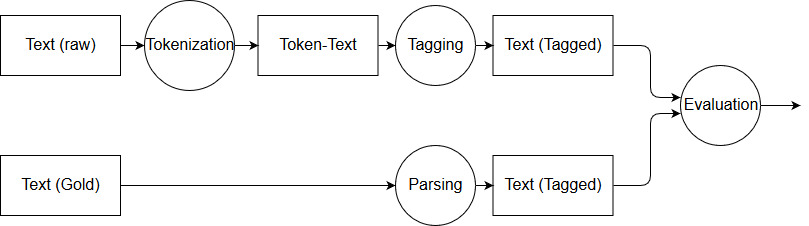
\includegraphics[width=\textwidth]{gfx/Dataflow_concept.jpg}
	\caption{Datenfluss für einen typischen Prozess von Rohdaten bis zur Evaluation}
	\label{fig:concept:overview}
\end{figure}

Aus Abbildung \ref{fig:concept:overview} können die Arbeitsschritte und Daten entnommen werden, die für Tagging und Evaluation modelliert werden müssen. Die folgenden Kapitel behandeln diese Schritte sowie insbesondere deren Eingaben und Ergebnisse.

\section{Sequenzierung}
\label{sec:concept:sequence}
Bei der Sequenzierung (\textit{Tokenization}) wird zwischen Wort- und Satzsequenzierung unterschieden \cite{Smith}. Satzsequenzierung beschäftigt sich mit einer Zerlegung des Textes in Sätze, welche für spätere Evaluation nützlich sein kann. Für Part-of-Speech-Tagging ist allerdings vorwiegend die Wort-Sequenzierung wichtig, da jedem Element der Wort-Sequenz ein Token zugewiesen wird. Außerdem sollte eine Satz-Sequenzierung vor dem Tagging nicht unbedingt stattfinden, da Tagger ggf. Kontextinformationen aus anderen Sätzen nutzen könnten, was die Auflösung von Ambiguitäten weiter unterstützen könnte. Allerdings verlangen manche Tagger eine Satzsequenzierung \cite{paroubek}.

Da Sequenzierunges-Algorithmen nicht standardisiert sind \cite{paroubek} und deren Ergebnisse von anderen - und insbesondere von Goldstandards - abweichen können, entstehen Unsicherheiten beim Vergleich dieser Sequenzen. 

\subsection{Tokenization-Unterschiede}
\label{sec:concept:sequence:tok}

Ein Token ist ein Abschnitt, zu dem ein Tag gehört, typischerweise einzelne Wörter oder Satzzeichen. Formal wird aus dem zusammenhängenden eingelesenen Wort beziehungsweise Text \textit{w} eine Menge \textit{M} von \textit{n} Teilwörtern c\textsubscript{i} 
 \[  M = \{ c_1 , c_2 , ... , c_n \} \] 
 generiert. POS-Tagger wie der von NLP4J \cite{choi} und der Stanford University \cite{Paper:StanfordTagger} können eine solche Zerlegung selbst übernehmen. Nehmen wir nun an, \textit{M} wäre die Zerlegung von \textit{w} in einem Goldstandard, und ein Tagger produziert ein Ergebnis mit der Zerlegung:
 \[  M_{tag} = \{ d_1 , d_2 , ... , d_m \} \]
Hierbei sind \textit{d\textsubscript{i}} wieder Teilworte und \textit{m} die Anzahl dieser. Spätestens wenn nun $n \neq m$ gilt, wird klar, dass \textit{M} und \textit{M\textsubscript{tag}} nicht mehr einfach iterativ verglichen werden können, da ab der Stelle \textit{p}, wo der Text unterschiedlich geteilt wurde, $ c_i \neq d_i $ sein kann, wobei $ (p \leq i \leq min\{ n, m \}) $. Es ist sogar nicht auszuschließen, dass solche Fehler bereits vorher passieren, obwohl weiterhin $n = m$ gilt.
\newline
Eines der Ziele bei der Implementierung ist also, den Vergleich von inhomogenen Token-Mengen robust gegen solche Fehler zu machen. 

\subsection{Externe Tokenization}
Um alternativ Probleme wie im vorigen Abschnitt zu verhindern, kann alternativ die Sequenzierung extern übernommen werden. D.h. dass den Taggern der Text bereits als Token-Kette übergeben wird. Hierzu muss entweder ein Tokenizer entwickelt werden, der den Taggern Tokens übergibt, die mit ihrem verlangten Format konform sind, oder im Falle eines Goldstandards kann die Token-Zerlegung aus dem annotierten Korpus selbst entnommen werden.
\\ Die meisten (alle implementierten) Tagger unterstützen das einlesen von bereits zerlegten Texten.



\section{Ergebnisformat}
\label{sec:concept:format}
Abhängig vom Tagger können Ergebnisse sehr Informationsreich sein. Der LingPipe-POS-Tagger liefert beispielsweise pro Token (Wort oder Symbol) nicht nur nicht nur das aus seiner Sicht plausibelste Tag (\textit{First-Best}), sondern auch \textit{n-1} weitere, nachstehende Optionen (\textit{N-Best}), wobei \textit{n} gewählt werden kann \cite{Lingpipedoc} . Eine solche Menge an Metainformationen kann möglicherweise von bereitgestellten Datenstrukturen seitens RapidMiner nur schwer kodiert werden. Eine speziell für Ergebnisse entworfene Datenstruktur bietet neue Freiheiten:

\paragraph{Satz-Sequenzierung} der Tag- und Token-Kette anhand von bestimmten Satzzeichen, die bei der Wort-Sequenzierung immer als eigenes Token eingefügt werden, macht robuster gegen Verschiebungen im Ergebnis wie in Abschnitt \ref{sec:concept:sequence:tok} beschrieben: Wird Satz-weise verglichen und entstehen in den Sätzen Verschiebungen durch ungleiche Token-Zerlegungen, dann verschwindet dieser Fehler, sobald ein neues Segment betreten wird, da die neuen betrachteten Segmente wieder an gleicher Stelle beginnen.
\paragraph{Anreicherung} mit Zusatzinformationen ist möglich, da im Gegensatz zu einer einfachen Textuellen Darstellung auf ein Token nicht exakt ein Tag folgen muss. Hier kann beispielsweise pro Token statt nur dem First-Best-Tag eine beliebig lange Liste der \textit{N-Best} Tags stehen.

Ein solches alternatives Format ist jedoch von Operatoren, die nicht speziell dafür vorbereitet sind (wie der Evaluationsoperator), nicht lesbar. Darum müssen Ergebnisse auch noch in einem Text-Format ausgegeben werden.

\section{Parsing von Ergebnissen}
Muss bei der Evaluation ein Text-Format angenommen werden, beispielsweise das Ergebnis in einem Goldstandard, muss entweder das angenommene Format exakt bekannt und definiert sein, oder das Dokument muss auf POS-Tags durchsucht werden. Letzteres bedeutet, dass dem Parser das Tagset des angenommenen Dokuments bekannt sein muss. Hierzu muss also jedes möglicherweise auftretende Tagset definiert werden.

\section{Evaluation}
\label{sec:concept:eval}
Um die Performance eines Taggers zu bewerten, müssen Metriken eingeführt werden. Diese entstehen aus Vergleichen zwischen annotierten Korpora und den Tagging-Ergebnissen. Im Rahmen dieses Projekts wird nur der Vergleich von Ergebnissen mit identischen Tagsets betrachtet. Abbildungsfunktionen zwischen Tagsets oder zu einem übergeordneten, generalisierten Tagset sind prinzipiell (mit einem gewissen Informationsverlust) möglich, werden aber hier außen vor gelassen. Betrachtet werden die folgenden Metriken zur Evaluation von Tagging-Ergebnissen:



\subsection{Per-Tag-Accuracy}

Die Per-Tag-Accuracy (ab hier nur \textit{Accuracy}) ist die wichtigste und einfachste Form der Bewertung eines Taggers. Sie ist definiert als \cite{Rao} :

\[ \frac{\# \: korrekter \:  Tags}{\# \: aller \:  Token} \]

\subsection{Per-Sentence-Accuracy}

Analog zur Accuracy pro Tag kann auch Accuracy pro Satz definiert werden:

\[ \frac{\# \: vollständig \: korrekter \:  Sätze}{\# \: aller \:  Sätze} \]

Hierzu müssen jedoch über Wort-Sequenzen hinaus auch Satz-Sequenzen definiert werden. Das fällt jedoch relativ leicht, da man die Sätze einfach nach jedem Satzzeichen-Token abschließen kann.

\subsection{Confusion Matrix und daraus resultierende Metriken}
Konzentrieren wir uns auf bestimmte Tags (Labels), können wir genauere Aussagen Treffen
(Für allgemeine Definitionen siehe \cite{Rao}, für mehrklassige Klassifizierungsprobleme siehe \cite{Web:rxnlp}). Zuerst bilden wir die \textit{Confusion Matrix}. In Abbildung \ref{fig:intro:pos:metrics:confusion} befindet sich ein Beispiel dafür. In dieser Matrix wird gegenübergesetzt, wie viele Labels aus dem Goldstandard als welche Labels vom Tagger vorhergesagt wurden.
\begin{description}

\item[True Positives] für Label X (kurz TP(X)) sind Vorhersagen, die dem Goldstandard entsprechen (in der Abbildung Gelb markiert).
\item[False Positives] (FP(X)) sind alle Vorhersagen X, die dem Goldstandard widersprechen.
\item[True Negatives] (TN(X)) sind alle Vorhersagen, die nicht X sind, und auch im Goldstandard nicht X lauten.
\item[False Negatives] (FN(X)) sind alle Vorhersagen, die nicht X sind, im Goldstandard aber X.
\end{description}

\begin{figure}[htb]
	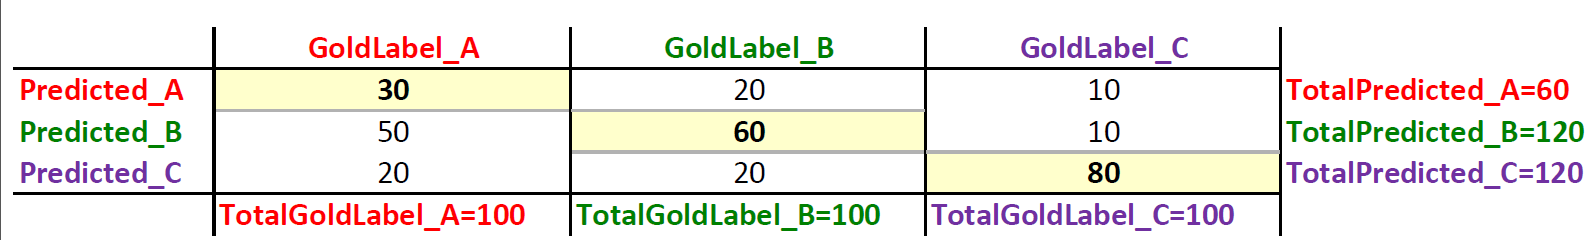
\includegraphics[width=\textwidth]{gfx/multi-class-confusionmatrix.png}
	\caption{Beispiel für eine Confusion Matrix für Labels A, B, C. Entnommen von \cite{Web:rxnlp}}
	\label{fig:intro:pos:metrics:confusion}
\end{figure}

Daraus lassen sich Precision(Wie viele der Vorhersagen X waren korrekt?), Recall(Wie viele X im Goldstandard wurden korrekt erkannt?) und der F1-Score(auch F-Score, harmonisches Mittel aus Precision und Recall) berechnen:
\[ Precision(X) \: = \: \frac{TP(X)}{TP(X)+FP(X)}\: = \: \frac{Korrekte\:X}{Vorhergesagte\:X} \]
\[ Recall(X) \: = \: \frac{TP(X)}{TP(X)+FN(X)} \: = \: \frac{Korrekte\:X}{X\:im\:Goldstandard} \]
\[ F1\mbox{-}Score \: = \: 2*\frac{Precision(X)*Recall(X)}{Precision(X)+Recall(X)} \]

Für alle drei dieser Metriken steht der Wert 1 für vollständig richtig und 0 für vollständig falsch.


\section{Zusammenfassung}
\label{sec:concept:conclusion}

In der Implementierung muss dafür gesorgt werden, dass Sequenzierungsunterschiede minimal bis gar nicht vorhanden sind, um Problemen bei der Evaluation vorzubeugen. Dies kann dadurch geschehen, dass die Sequenzierung vorweg stattfindet und den Taggern bereits sequenzierter Text übergeben wird. Es wurde festgestellt, dass zum erfolgreichen Parsen von Goldstandards und Ergebnissen die Tagsets definiert werden müssen. Zusätzlich wurde eine Datenstruktur beschrieben, mit der möglichst viele Informationen zum Tagging-Ergebnis beigelegt werden können. Letztlich wurden die Evaluationsmetriken definiert, mit denen wir die Qualität eines Ergebnisses beurteilen können.

Mit diesen Definitionen und Feststellung können wir uns nun der der tatsächlichen Planung und Implementierung der Erweiterung zuwenden.
 % INCLUDE: concept
% !TEX root = ../thesis-example.tex
%
\chapter{Implementierung}
\label{sec:impl}

Dieses Kapitel behandelt die Implementierung der RapidMiner-Erweiterung \textit{postagger}. Zuerst wird grob auf den technischen Rahmen seitens RapidMiner eingegangen, dann werden im Abschnitt \ref{sec:impl:aims} Ziele der Implementierung angesprochen. \\
Nach einer Übersicht in Abschnitt \ref{sec:impl:structure} über die Komponenten, die Funktionen aus Kap. \ref{sec:concept} implementieren, werden die Komponenten einzeln im Detail vorgestellt.

\section{RapidMiner}
\label{sec:impl:rm}


Die Datenverarbeitungs-Plattform RapidMiner (kurz \textit{RM}) und ihre Erweiterungen sind in Java geschrieben. RapidMiners zentrale Funktionalität ist es, verschiedene Funktionen (\textit{Operatoren}) in einem Modell hintereinanderzuschalten und mit ihnen Daten zu extrahieren und mit verschiedensten Mitteln zu transformieren oder zu untersuchen.

\paragraph{Operatoren} 
funktionieren entfernter betrachtet wie Funktionen in Programmen: Sie nehmen beliebig viele Eingaben mittels \textit{InputPorts} und \textit{Parametern} entgegen, führen eine Aufgabe aus und haben mindestens eine Ausgabe in Form von \textit{OutputPorts}. Alle Operatoren erben von der Superklasse \textit{Operator}. Eine Erweiterung fügt in der Regel solche Operatoren hinzu.
\paragraph{IO-Objekte}
bzw. IOObjects sind die Datenformate im RM-Modell. Sie werden von der Prozesswurzel sowie von Operatoren ausgegeben und können von Operatoren sowie dem Prozess-Ende entgegengenommen werden. Sie erben von der Klasse \textit{IOObject} und können ebenfalls von Erweiterungen hinzugefügt werden. Operatoren können für ihre Inputs definieren, welche Typ von IOObject sie verlangen. Das Prozessmodell ist nicht lauffähig, wenn diese Spezifikation nicht eingehalten wird.

Eine ausführliche Dokumentation von RM findet sich in \cite{rmdoc} und eine Anleitung zum Erstellen von Erweiterungen bei \cite{rmext}.
 Die implementierte Erweiterung baut auf der Erweiterung \textit{Text Processing} auf, die mit ihren Operatoren und insbesondere dem Übergabeobjekt \textit{Document} (fortan auch einfach als Dokument bezeichnet) viel Arbeit übernimmt. Das Format Document ist prinzipiell nur ein Container für Texte, wobei mit den Operatoren von \textit{Text Processing} bereits viel auf diesem Text gearbeitet werden kann. Zusätzlich sind diese Dokumente bereits in der Lage, Sequenzierungen zu kodieren.
 
 Freundlicherweise wurde von der Firma RapidMiner GmbH eine Arbeitslizenz für dieses Projekt zur Verfügung gestellt.

\section{Ziele}
\label{sec:impl:aims}
Diese Erweiterung soll u.A. vom auftraggebenden Lehrstuhl weiterverwendet und -entwickelt werden können. Das heißt, eine gute Dokumentation und Strukturierung der Komponenten steht im Vordergrund. Da die Erweiterung nicht unbedingt von Programmierern benutzt werden soll, muss außerdem auf eine niedrige Fehleranfälligkeit der Implementierung geachtet werden.
\subsection{Erweiterbarkeit}
Mit Hilfe von Interfaces, Superklassen und statischen Methoden soll gewährleistet sein, dass durch das Hinzufügen von Komponenten nur minimale bis keine Änderungen an anderen nötig sind.
\subsection{Robustheit}
Verwendung von Operatoren außerhalb ihres Funktionsbereiches soll entweder von vornherein unmöglich sein oder leicht verständliche und eindeutige Fehlermeldungen ausgeben. Auch der Vergleich von nicht identischen Ergebnissen soll weitgehend unterstützt werden und Probleme, wie in Kap. \ref{sec:concept:sequence:tok} beschrieben, sollten abgefangen werden.

\section{Übersicht}
\label{sec:impl:structure}

 
\begin{figure}[htb]
	\captionsetup{justification=centering,margin=2cm}
	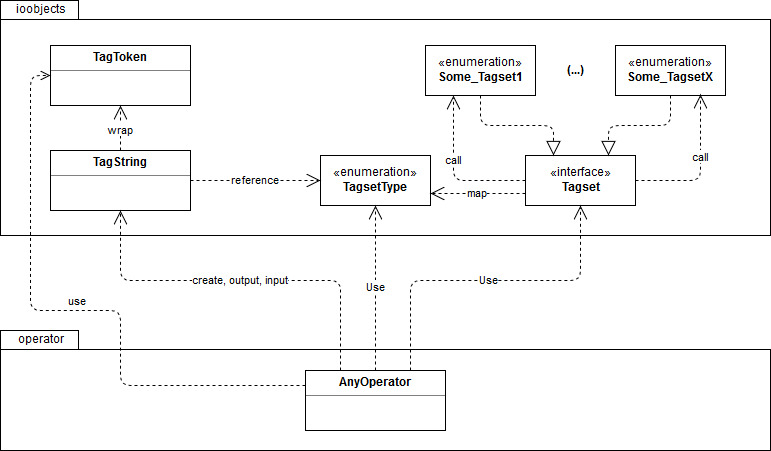
\includegraphics[width=\textwidth]{gfx/uml_rough.jpg}
	\caption{Gekürztes Klassendiagramm der Erweiterung mit Beziehungen}
	\label{fig:impl:structure:overview}
\end{figure}

Abbildung \ref{fig:impl:structure:overview} zeigt einen groben Überblick. Es wurden nur Beispiel-Operatoren und -Tagsets eingezeichnet, sodass nur das Konzept verdeutlicht wird. Es folgt eine kurze Erklärung der verschiedenen Komponenten:

\paragraph{Operatoren} sind Klassen, die von der RapidMiner-Klasse \textit{Operator} erben, und sind auch in der RapidMiner-Nutzeransicht direkt als solche Operatoren vertreten. Alle Operatoren außer dem \textit{Evaluator} beinhalten einen POS-Tagger und wandeln Ein- als auch Ausgangsformate zwischen dem externen RapidMiner-Modell (\textit{Document} oder \textit{TagString} ) und den Vorgaben des Tagging-Algorithmus selbst um. Der Evaluator selbst berechnet die in Kap. \ref{sec:concept} vorgestellten Evaluationsmetriken durch Vergleich von zwei Ergebnissen. Die genaue Funktionsweise des Evaluators wird in Abschnitt \ref{sec:impl:eval} vorgestellt.

\paragraph{Tagsets:} Das Interface Tagset muss von jeder Tag-Enumeration, wie zum Beispiel der des Penn-Treebank-Tagsets implementiert werden. Zusätzlich bietet es statische Methoden, die die Werte der Enumeration TagsetType auf die korrespondierenden Enumerationen abbilden, sowie Abfragen über deren Werte anbieten (hierzu wird der Typ sowie ein Tag verlangt). Auf diese Weise kann ein Tagset mit nur seinem Typen adressiert werden und es ist leicht, das Projekt um ein neues Set zu erweitern.

\paragraph{TagString:} Diese Klasse bietet, wie in Abschnitt \ref{sec:concept:format} angesprochen, ein einheitliches Format für mit Tags versehene Token-Ketten. Sie beschreibt den Tagset-Typen sowie die Zahl an N-Besten Tags pro Token und strukturiert die Tags in Zeilen, die immer dann enden, wenn das letzte Token ein \textit{Separator} ist. 

\section{Tagsets}
\label{sec:impl:tagset}


\begin{figure}[htb]
	\centering
	\captionsetup{justification=centering,margin=2cm}
	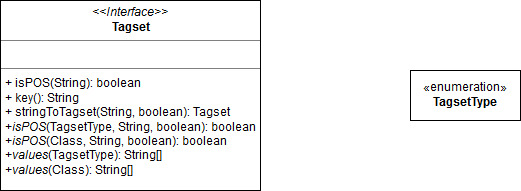
\includegraphics[width=0.7\textwidth]{gfx/tagset_uml.jpg}
	
	\caption{Klassendiagramm-Abschnitt: Tagsets (ohne Beziehungen)} 
	\label{fig:impl:tagset:uml}
\end{figure}

Das Interface \textit{Tagset} realisiert die Aufführung von POS-Tagsets.
Jede Enumeration, die Tagset implementiert, führt eine Gruppe an Tags, wie zum Beispiel die der \textit{Penn Treebank} \cite{Paper:PennBank}, auf und wird von einer Konstante in \textit{TagsetType} repräsentiert. Um eine korrekte Evaluation zu ermöglichen, müssen alle Tags, die auftreten können, in der entsprechenden Enumeration vertreten sein (Der Evaluationsmechanismus zählt nur bekannte Tags als potenziell korrekt). Hat ein Tagger eigene definierte Tags, die vom Standard abweichen, sollten auch diese hinzugefügt werden. Die Enumeration muss folgende Funktionen implementieren:
\begin{description}
\item[key()] liefert den Key des gewählten Tags zurück (falls der Name der Enumerations-Konstante nicht gleich dem Tag ist, würde toString() nicht funktionieren).
\item[isPOS(String key)] liefert genau dann \textsc{true} zurück, wenn ein Tag mit dem übergebenen Key existiert und es ein POS-Tag ist.
\item[stringToTagset(String key, boolean strict)] liefert die Enumerationskonstante für ein Tag mit dem übergebenen Key zurück, sofern es existiert. Falls \textsc{strict} gesetzt ist, wird die Groß- und Kleinschreibung beachtet.
\end{description}

\subsubsection{Mapping von TagsetType auf Tagsets}

Die überladenen statischen Methoden \textit{IsPOS} und \textit{values} haben jeweils eine Variante mit dem Parameter TagsetType, und eine mit dem Parameter Class. Die TagsetType-Variante ersetzt den Tagset-Typen durch seine korrespondierende Enumeration und ruft dann die andere Variante auf. Die andere Variante operiert dann auf dieser Klasse.

Sinn dieser Aufteilung ist es, dass ein Aufruf nicht mit einer Enumeration oder ihrer Implementierung interagieren muss, sondern sie nur via TagsetType adressiert. Wenn eine Änderung an den implementierenden Tagsets vorgenommen wird, muss diese nur im Interface und in TagsetType bekannt werden. Dadurch senkt sich der Aufwand für eine solche Änderung extrem und die Erweiterbarkeit ist für die Menge der Tagsets gewährleistet.

\begin{description}
\item[isPOS(...) (statisch)] gibt die Ergebnisse von der Methode isPOS() der entsprechenden implementierenden Enumeration aus.
\item[values(...) (statisch)] sammelt alle Keys einer implementierenden Enumeration für die isPOS() mit gesetztem \textsc{strict} gilt.
\end{description}

\section{Eingabe und Tokenization}
Zum Einlesen von Text werden bereitgestellte Operatoren von der Erweiterung \textit{Text Processing} (z.B. \textit{read Document}) verwendet. Für diese Aufgabe wurden deshalb keine eigenen Operatoren implementiert. (Satz- und) Wortsequenzierung, wie in \ref{sec:related:pos} definiert, wird ebenfalls von \textit{Text Processing} bereits unterstützt. Hierzu kann ein eingelesenes Dokument einfach mit dem Operator \textit{Tokenize} verarbeitet werden. Eine optimale Sequenzierung liefert der Operator, wenn die Einstellung \textsc{(mode = linguistic tokens)} gesetzt ist.

 Dokumente, die bereits in Tokens zerlegt sind, können mit der Methode \textsc{Document\# getTokenText(): String} abgerufen werden und geben die Token mit Leerzeichen getrennt zurück. Dieses Format ist dann leicht in andere Formate, wie z.B. Listen, zu zerlegen. Um, wie in Abschnitt \ref{sec:concept:sequence} erklärt, Sequenzierungsprobleme zu verhindern, wird Sequenzierung in den Tagging-Operatoren gezielt weggelassen und stattdessen wird ein Davorschalten des Operators \textit{Tokenize} wie oben beschrieben verlangt.

\section{Tag-String als Ergebnisformat}
\label{sec:impl:tagstring}

\begin{figure}[htb]
	\centering
	\captionsetup{justification=centering,margin=2cm}
	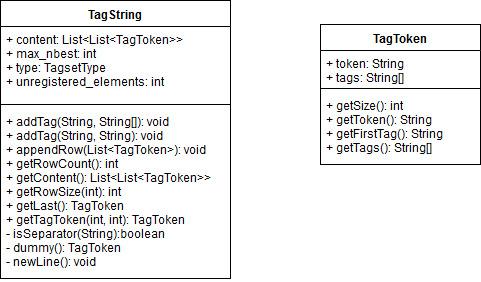
\includegraphics[width=0.7\textwidth]{gfx/tagstring_uml.jpg}
	
	\caption{Klassendiagramm-Abschnitt: TagString (ohne Beziehungen)} 
	\label{fig:impl:tagstring:uml}
\end{figure}

Das in \ref{sec:concept:format} konzeptuell eingeführte Ergebnisformat wird von der Klasse \textit{TagString} realisiert. Solche TagString-Objekte werden vom Parser des Evaluations-Operators (siehe Abschnitt \ref{sec:impl:eval:parsing}) und von Tagging-Operatoren erzeugt und vom Evaluator verwendet. TagStrings sind vorwiegend dazu entworfen, Iteration über Tag-Token-Ketten zu erleichtern und Sequenzierungsfehlern zu entgehen.

\subsection{Metainformationen}
Der TagString bietet die Möglichkeit, beim Erzeugen seinen Tagset-Typen \textsc{[TagsetType type]} festzulegen und zu definieren, wie viele N-Best (Variable \textsc{[int max\_nbest]}) Tags pro Token gespeichert werden sollen. Wird beim Hinzufügen eines Tokens die falsche Menge an Tags hinzugegeben, stellt der TagString von selbst sicher, dass so viele überflüssige Tags entfernt bzw. ungültige Tags hinzugefügt werden, dass die angegebenen \textsc{max\_nbest} Tags vorhanden sind. Der Tagset-Typ wird genutzt, um mittels der statischen Methoden von \textit{Tagset} zu prüfen, ob hinzugefügte Tags (bei mehreren pro Token nur das erste) Teil ihres Tagsets sind. Falls nicht, wird das Tag zwar hinzugefügt, aber der Zähler \textsc{[int unregistered\_elements]} wird inkrementiert.
\subsection{TagToken}
Die TagToken-Objekte sind die Elemente der TagString-Struktur. Sie enthalten ein Token und ein Array an Tags, wobei das erste Tag im Array das First-Best Tag ist. Die Bestandteile können mit den entsprechenden \textsc{get}-Methoden abgefragt werden. Die Methode \textsc{[getSize(): int]} liefert die Größe des Tag-Arrays zurück.

TagTokens wurden eingeführt, um Informationen hinzufügen zu können, ohne Änderungen im restlichen Code zu veranlassen.
\subsection{Aufbau des TagStrings}

Die verschachtelte Liste \textsc{content}, die die TagToken-Objekte sortiert, übernimmt nicht nur die Wort-, sondern auch Satzsequenzierung der Tagging-Ergebnisse. Die innere Liste stellt Sätze dar und wird von der äußeren in Reihenfolge gebracht. 

\subsubsection{Adressierung von Token}
Um das Iterieren über \textsc{content} zu ermöglichen, ohne die Struktur selbst kopieren zu müssen, wurden Hilfsmethoden implementiert. Mit \textsc{getRowCount()} wird die Zahl an Sätzen und mit \textsc{getRowSize(int)} die Zahl an TagToken in einem spezifizierten Satz abgefragt. Mit diesen Informationen kann jedes TagToken via \textsc{getTagToken(int, int)} ausgegeben werden. Ist die Adressierung falsch, wird \textsc{dummy()} aufgerufen, um ein neues TagToken mit ungültigen Tags ("NONE") zurückzugeben. Dadurch sind Iterationen robuster gegen Fehler.

\subsubsection{Serialisierung}
Falls die Zerlegung in Sätze nicht erwünscht ist, kann sie mit der Methode \textsc{serialize()} aufgelöst werden. Dann werden alle inneren Listen zu einer zusammengefasst.

\subsubsection{Hinzufügen von Token}
Beim Hinzufügen von Tagging-Ergebnissen mittels \textsc{addTag(...)} prüft der TagString selbstständig mit Hilfe der Methode \textsc{isSeparator()}, ob das hinzugefügte Token ein Zeilenseparator ist. Als solche Separatoren werden von der Hilfsmethode alle Token identifiziert, die mit Satzzeichen (Punkt, Fragezeichen etc.) beginnen. Ist dies der Fall, wird automatisch die aktuelle Zeile beendet und eine Neue begonnen. 

Den Zeilenumbruch übernimmt der TagString selbst, um eine gleiche Satzsequenzierung verschiedener Ergebnisse zu garantieren, sofern bei diesen die Wortsequenzierung entweder identisch ist oder zumindest jedes Satzzeichen korrekt als eigenes Token abgespalten wurde.

\section{Implementierte Tagging-Operatoren}
Jeder implementierte Tagging-Operator hat folgendes In- und Outputverhalten: Eingelesen wird ein sequenziertes Dokument (es reicht aus, wenn jedes Token durch ein Leerzeichen von Vorgänger und Nachfolger getrennt ist), und ausgegeben dasselbe Dokument, wobei nach jedem Token ein \glqq \ \grqq{} und das Tag folgen. Zusätzlich wird das Tagging-Ergebnis im Format TagString ausgegeben.

\paragraph{NLP4J}
(Dokumentation: \cite{choi}) ist der laut eigenen Angaben leistungsfähigste der implementierten POS-Tagger. Er kann bei der Initialisierung mit trainierten Modellen und Lexika konfiguriert werden. Das eröffnet die Möglichkeit, diese Modelle per Parameter wählbar zu machen, oder sogar via Text-Parameter eigene Modelle und Lexika einzufügen. In dieser Implementierung sind Modell und Lexikon jedoch festgesetzt.
\paragraph{LingPipe}
(Dokumentation: \cite{Lingpipedoc})ist, wie der NLP4J-Algorithmus, mit einem Modell initialisierbar. Die drei verschiedenen vortrainierten Modelle, die der Implementierung beigefügt wurden, sind zu Demonstrationszwecken alle in einem Parameter wählbar gemacht worden. Allerdings liefert nur das Modell, das auf dem \textit{GENIA Korpus} \cite{GENIA} trainiert wurde, POS-Tags zurück, die dem \textit{Penn Treebank} Tagset entsprechen. Da der Evaluations-Testlauf in Kapitel \ref{sec:eval} sich nur auf letzteres Tagset bezieht, sind andere Tagsets noch nicht als entsprechende Enumerationen implementiert.
\paragraph{FastTag}
(Quellcode und Dokumentation: \cite{fasttagdoc})ist ein simpler, nicht auf Trainingsdaten beruhender POS-Tagger. Er wurde implementiert, um einen Vergleich zu den anderen, lernenden POS-Taggern zu bieten.




\section{Evaluations-Operator}
\label{sec:impl:eval}
Der Operator \textit{Evaluator} ist die Zentrale Komponente dieser Erweiterung. Er muss die Formate von Goldstandards sowie Tagging-Ergebnisse annehmen und interpretieren können. Neben dem eigentlichen Evaluieren ist also auch das \textit{Parsen} eingehender Texte eine wichtige Aufgabe des Operators. 

\subsection{Parsing von Ergebnissen}
\label{sec:impl:eval:parsing}
Werden Ergebnisse als Typ Document ausgegeben oder wird ein Goldstandard mit Operatoren aus \textit{Text Processing} eingelesen, liegt ein Document-Objekt mit einem Kodierungsformat vor. Dieses Dokument muss mittels Parsing-Techniken in das TagString-Format transformiert werden, damit eine Evaluation darüber stattfinden kann.

Verschiedene Formate kodieren POS-Tags unterschiedlich. Eine einfache Notation ist die bereits aus der Einleitung bekannte Variante, bei der nach jedem Token ein \glqq \textbackslash \grqq{} und dann das Tag folgt. Andere Notationen kodieren zusätzlich Satzstrukturinformationen, sind also geschachtelt, um z.B. Teilsätze zu markieren. Hier gibt es kein Symbol, das eindeutig ein POS-Tag ankündigt. Um die Parser-Methode des Evaluationsoperators präziser arbeiten können zu lassen, wurde ein Parameter hinzugefügt, in dem man das eingelesene Format und damit den Modus des Parsers nennen kann. Es wurden drei Modi (und damit wählbare Parameter) für den Parser implementiert:

\paragraph{Backslash-Notation:} \cite{Smith} In der oben genannten Notation, in der ausschließlich POS via \glqq \textbackslash \grqq{} markiert werden, ist Parsing einfach. In dieser Notation wird jedes Token mit einem Leerzeichen von seinem Vorgänger und Nachfolger getrennt. Letztlich muss nur noch die Struktur
\[ WORD \mbox{\textbackslash} TAG\]
gefiltert werden.

\paragraph{Parenthesis-Notation bzw. Penn-Treebank-Standard:} \cite{Paper:PennBank} In dieser Notationsvariante wird mittels Klammern die Satzstruktur zerlegt. Wichtig ist, dass Token und Tags immer im Format \textsc{(TAG TOKEN)} bzw. \textsc{(TOKEN TAG)} auftreten. Ferner kann ein Tag also nur auftreten, wenn die Struktur
\[ "(" \: WORD \:\: WORD \: ")" \]
erscheint. Es ist sogar anzunehmen, dass diese Struktur \textit{ausschließlich} Token-Tag-Kombinationen kodiert. Der Parser muss also nur diese Struktur finden und identifizieren, ob eines der beiden Worte ein gültiges POS-Tag ist.

\paragraph{None:} Falls die Notation unbekannt ist, versucht der Parser, den Text an allen sinnvollen Symbolen, insbesondere dem Leerzeichen, zu trennen. Alle Substrings werden dann überprüft, ob sie ein POS-Tag sind. Hier können die Token allerdings nicht identifiziert werden und es handelt sich nur um eine Ausweichs-Option. 

Ein neuer Parsing-Modus kann der Methode einfach hinzugefügt werden. Zusätzlich kann die Option \textit{\glqq Ignore Brackets\grqq{}} gewählt werden, falls Klammern für die Formatierung des einzulesenden Textes verwendet wurden (In der Parenthesis-Notation erübrigt sich das), diese werden dann ignoriert.
\\
Der Tagset-Typ des eingelesenen Dokuments und des ausgegebenen TagStrings muss via Parameter angegeben werden.

\subsection{Iteration über TagStrings}
\label{sec:impl:eval:comparison}

Vergleichsfunktionen müssen nur TagStrings entgegennehmen, da andere Formate vom Parser in solche umgewandelt werden. Aufgrund der automatischen Unterteilung von Token-Ketten in Sätze durch TagStrings kann nicht nur Token- sondern auch Satzweise verglichen werden. Iteriert wird also erst über die Sammlung an Sätzen, dann über deren individuelle Token.

Bei identischer Wort-Sequenzierung der beiden Ergebnisse erübrigen sich Überlegungen über die Robustheit des Vergleichsverfahrens. Hier kann davon ausgegangen werden, dass an gleichen Positionen im TagString auch gleiche Token platziert sind. Bei der Iteration werden also keine Probleme entstehen.

Bestehen allerdings Sequenzierungsunterschiede (siehe Abschnitt \ref{sec:concept:sequence}), kann korrektes Iterieren nicht mehr garantiert werden. Darum wird zuerst überprüft, ob die Satzsequenzierung übereinstimmt. Von einer korrekten Sequenzierung wird ausgegangen, wenn beide zu vergleichenden TagStrings dieselben Satz-Anahlen mit \textsc{countRows()} zurückliefern. Ist dies \textit{nicht} der Fall, muss die Satzsequenzierung aufgelöst werden. Dazu wird bei den TagStrings \textsc{serialize()} aufgerufen (Beschreibung siehe Abschnitt \ref{sec:impl:tagstring}). Danach wird wie zuvor iteriert, wobei beide TagStrings effektiv nur noch einzeilig sind, und Wort-Sequenzierungs-Unterschiede nicht abgefangen werden können. Ist die Satzsequenzierung hingegen korrekt, würden solche Unterschiede beim Iterieren über die Token allerdings nur Probleme innerhalb des Satzes verursachen, da beim nächsten untersuchten Satz die Iteration neu starten kann.

Daraus wird erkennbar, warum bei ungleicher Sequenzierung kein garantiert optimaler Vergleich mehr stattfinden kann. Für korrekte Sequenzierung muss also, wenn möglich, unbedingt schon vorher im Prozess gesorgt werden.

\subsection{Berechnung der Metriken}
\label{sec:impl:eval:calc}

Mittels dem erklärten Iterations-Vorgehen aus dem letzten Abschnitt und den Definitionen aus Abschnitt \ref{sec:concept:eval} kann die Berechnung der Evaluationsmetriken beim Vergleich zweier TagStrings leicht erklärt werden.

\subsubsection{Accuracy}
Per-Tag-Accuracy berechnet sich aus der Zahl der beim Vergleichen der TagStrings identischen Tags geteilt durch die Gesamtzahl der Token (bei ungleicher Satzlänge wird die größere Anzahl an Token zur Gesamtzahl hinzugerechnet). Die Per-Sentence-Accuracy besteht analog aus der Zahl absolut identischer Sätze, geteilt durch deren Gesamtzahl.

\subsubsection{Confusion-Matrix}
Die Confusion-Matrix wird wie folgt gebildet: Zuerst muss eine Liste der auftretenden Tags gebildet werden. Diese wird vom Interface \textit{Tagset} statisch angefragt. Die Matrix hat exakt so viele Zeilen und Spalten wie Tags und deren Index repräsentiert das entsprechende Tag in der Tag-Liste. Die Matrix-Positionen \textsc{matrix[X][Y]} repräsentieren Token, deren Goldstandard-Tag in der Tag-Liste Index X hat, und deren Ergebnis-Tag Index Y hat. Per Definition sind für Tag mit Index X die entsprechenden Werte also wie folgt zu berechnen (\textsc{I} sei hier der maximale Index der Tag-Liste):
\[True\: Positive\:(X)\:=\: matrix[X][X]\]
\[False\: Positive\:(X)\:=\: \Bigg(\sum_{i=0}^I matrix[i][X]\Bigg) - matrix[X][X] \]
\[False\: Negative\:(X)\:=\: \Bigg(\sum_{i=0}^I matrix[X][i]\Bigg) - matrix[X][X] \]
\textit{True Negatives} sind für die berechneten Metriken \textit{Precision, Recall und F-Score} nicht interessant. Precision und Recall sind dementsprechend:

\[Precision(X) \:=\: \frac{matrix[X][X]}{\sum_{i=0}^I matrix[i][X]}\]
\[Recall(X) \:=\: \frac{matrix[X][X]}{\sum_{i=0}^I matrix[X][i]}\]
 
Der F-Score wird wie in Kapitel \ref{sec:concept} definiert als harmonisches Mittel von Precision und Recall berechnet. Die Rechnung $\frac{0}{0}$ wird abgefangen, sodass stattdessen null als Ergebnis ausgegeben wird.

\subsubsection{N-Best Tags}
Wurde beim Parameter \textit{Calculate N-Best Distance} ein Haken gesetzt, werden zwei weitere Metriken berechnet:

\paragraph{N-Accuracy:} Diese Variante der Accuracy wird analog zur Per-Tag-Accuracy berechnet. Allerdings werden alle Tags pro Token im Tagging-Ergebnis mit dem korrekten Tag im Goldstandard verglichen. Findet sich unter allen Tags ein Korrektes, wird wie bei der normalen Per-Tag-Accuracy von einem korrekten Tag ausgegangen. Dieser Wert ist also mindestens so hoch wie die Per-Tag-Accuracy desselben TagStrings.
\paragraph{N-Distanz:} Um genauere Einsicht darauf zu liefern, an welcher Stelle das durchschnittliche korrekte Tag unter den besten n stand, wird die durchschnittliche Distanz eingeführt. Ist das erste Tag korrekt, beträgt die Distanz für dieses Token 1, ist das zweite korrekt, ist sie 2, und so weiter. Wird das  korrekte Tag unter den besten n nicht gefunden, lautet die Distanz n+1. Die N-Distanz für einen ganzen TagString ist dann der Durchschnitt aller Distanzen pro Token.

\subsection{Ausgabe}
\label{sec:impl:eval:out}

Da diese Erweiterung zur Weiterentwicklung konzipiert wurde und in eine größere Bilbiothek übernommen werden wird, wurde die Definition eines Evaluations-Formats absichtlich weggelassen.

Als Ersatz liefert der Evaluationsoperator ein Dokument aus, in dem alle berechneten Ergebnisse (und falls gewünscht auch die Confusion-Matrix) textuell wiedergegeben werden. Zusätzlich gibt ein zweiter Output das Ergebnis des Parsers beim eingelesenen Goldstandard aus, sodass überprüft werden kann, ob der Parsing-Prozess korrekt abgelaufen ist.

\section{Zusammenfassung}
\label{sec:system:conclusion}

Der Evaluationsoperator bietet Einsichten über verschiedene Evaluationsmetriken beim Vergleich zweier Tagging-Ergebnisse, wobei einer davon als Goldstandard betrachtet wird. Sind beide Ergebnisse kein Goldstandard, können die beiden \textit{Accuracy}-Werte als Übereinstimmung der Ergebnisse interpretiert werden. Als Tagging-Algorithmen wurden drei unterschiedlich konfigurierbare POS-Tagger in Operatoren verpackt. Während die Tagger ihre Ergebnisse in Textform ausgeben und der Evaluator diese einlesen können, wurde für eine informationsreichere Übergabe von Daten die Datenstruktur TagString definiert. Zusätzlich wurden die verwendbaren Tagsets als Enumerationen definiert.

Mehrere Methoden wurden angewendet, sodass die Erweiterung leicht um neue Tagsets oder Informationen im TagString vergrößern werden kann. Es wurde auch darauf geachtet, dass der Evaluationsoperator möglichst nicht fehleranfällig ist und im Falle eines Fehlers nützliche Informationen an den Nutzer ausgibt.	% INCLUDE: implementation
% !TEX root = ../thesis-example.tex
%
\chapter{Evaluation}
\label{sec:eval}



\begin{table}[htb]
\centering
\begin{tabular}{l|l|l}
Tagger (Trainingskorpus) & Performance(eigen) & Performance(test)  \\
\cline{1-3}
NLP4J(WSJ)  & 97.64\% & 94,86\%	\\
LingPipe(GENIA) & 96.9\% & 77,26\%	\\
FastTag(-) & - & 30,72\%          
\end{tabular}
\vspace{3mm}
\caption{Liste der Implementierten Tagger. }
\label{sec:eval:list}
\end{table}

In diesem Kapitel wird ein Test mit einem fremden Goldstandard an den implementierten Taggern ausgeführt. In Tab. \ref{sec:eval:list} sind die Per-Tag-Accuracies der Tagger aufgeführt. Performance(eigen) ist die Per-Tag-Accuracy laut eigenen Angaben (Quellen in den weiterführenden Abschnitten), Performance(test) die Per-Tag-Accuracy in diesem Test. Es ist hierbei jedoch unbedingt anzumerken, dass in diesem Test \textit{keine} Vergleiche zwischen den Taggern gezogen werden können. Hierzu müssten alle Tagger, bei denen dies möglich ist, auf den Korpus trainiert werden, um den \textit{Bias} der Tagger anzugleichen und die Ergebnisse für diesen speziellen Korpus dadurch vergleichbar zu machen.

Allerdings kann man aus einem Vergleich der eigenen Angaben mit den Testergebnissen sehen, wie stark die Performance-Änderung ist, wenn man dem Tagger einen fremden Korpus zuführt. Da auch die Trainingskorpora der Tagger sich unterscheiden, kann allerdings auch diese Änderung nicht als Vergleich zwischen den Taggern genutzt werden.

Die folgenden Abschnitte diskutieren die Auswahl eines passenden Korpus und die Performance (\textit{Scores}) der Tagger auf diesem.

\section{Goldstandard-Korpus und Aufbau des Tests}
\label{sec:eval:corpus}

Ein annotierter Korpus muss natürlich dem Tagset der einzelnen zu testenden Tagger entsprechen. Zudem sollte aus dem Goldstandard direkt die Sequenzierung auslesbar sein, da sonst Tokenization stattfinden müsste und Sequenzierungsunterschiede die Ergebnisqualität der Tagger trüben könnten.

Ein Korpus, der beiden Kriterien entspricht, ist die \textit{NAIST/NTT TED Treebank} \cite{tedbank}. Alle Inhalte sind sowohl als \textit{Tokenized} (Token getrennt durch Leerzeichen und Zeilenumbrüche) als auch annotiert nach derselben Sequenzierung verfügbar. Die zur POS-Tag-Evaluation überflüssigen Syntaxbaum-Tags können einfach ignoriert werden. Die Notation des Annotierten Textes entspricht der Klammer-Notation  aus Abschnitt \ref{sec:impl:eval:parsing} und kann somit vom Parser des Evaluationsoperators erkannt werden.

Im Rahmen des Tests wird diese Treebank verwendet. Der RapidMiner-Prozess zum Testen ist in Abb. \ref{fig:eval:corpus:process} dargestellt. Für die nachfolgenden Tests wurden sämtliche Teilstücke des Testkorpus eingelesen und zu einem Dokument aneinandergereiht. Zur Übersichtlichkeit wurde in der Abbildung allerdings nur einfaches Einlesen von einem Teilstück modelliert. 

\begin{figure}[htb]
	\centering
	\captionsetup{justification=centering,margin=2cm}
	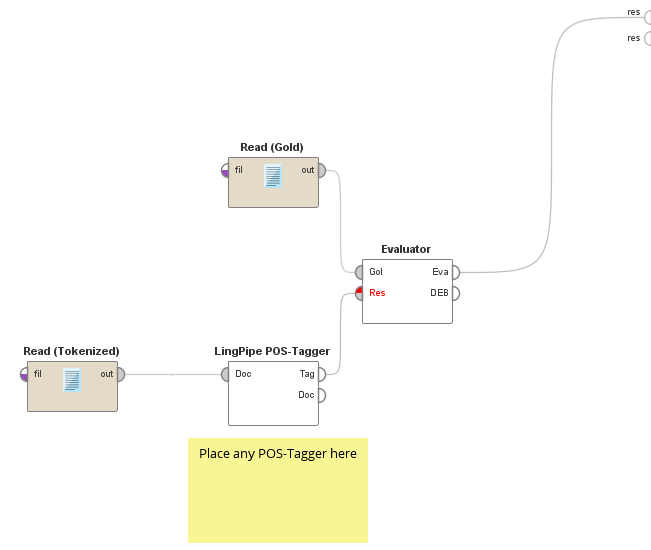
\includegraphics[width=0.7\textwidth]{gfx/process.png}
	
	\caption{Aufbau des Test-Evaluationsprozesses} 
	\label{fig:eval:corpus:process}
\end{figure}

Der LingPipe-Tagger im Prozess hat identische Inputs und Outputs zu den anderen Taggern und kann hier einfach ersetzt werden. Die Einlese-Operatoren lesen für den Tagger die sequenzierten Texte mit der Dateiendung \textsc{.tok} und als Goldstandard die annotierten Texte in Klammer-Format mit Endung \textsc{.mrg}. Der Evaluationsoperator \textit{Evaluator} wird auf diese Formatierung konfiguriert.

\section{Evaluation der einzelnen Tagger}
\label{sec:eval:detail}

\subsection{NLP4J (WSJ)}
\label{sec:eval:detail:nlp4j}

\begin{table}[htb]
\centering
\captionsetup{justification=centering,margin=2cm}
\begin{tabular}{l|l}
Metrik & Performance \\
\cline{1-2}
Per-Tag-Accuracy & 94,86\%\\
Per-Sentence-Accuracy & 49,19\%\\
\cline{1-2}
Precision(NN) & 96,11\%\\
Recall(NN) & 96,85\%\\
F-Score(NN) & 96,48\%\\
\cline{1-2}
Precision(VBD) & 95,11\%\\
Recall(VBD) & 95,7\%\\
F-Score(VBD) & 95,4\%
\end{tabular}
\vspace{3mm}
\caption{Scores des NLP4J-Taggers (Training: WSJ-Korpus)}
\label{tab:eval:detail:nlp4j}
\end{table}

Der NLP4J-Tagger erreicht gemäß der Werte in Tab. \ref{tab:eval:detail:nlp4j} beinahe seine maximale Leistungsfähigkeit(97.64\% \cite{choi}). Daraus lässt sich schließen, dass der \textit{Bias} in Richtung des WSJ-Korpus, auf dem trainiert wurde, zu keinen sehr hohen Performanceverlusten beim Testkorpus führt, also eine hohe Ähnlichkeit zwischen den Korpora herrscht. Alternativ könnte der NLP4J-Tagger auch hochgradig unanfällig gegen Bias sein, allerdings müssten für solch eine Aussage mehr Tests stattfinden. 

Auffällig ist die Per-Sentence-Accuracy von knapp 50\%, jedoch klärt eine kurze Rechnung das schnell auf: Bei einer Wahrscheinlichkeit von 94,86\% und einer (angenommenen) durchschnittlichen Satzlänge von 13 Wörtern beträgt die Wahrscheinlichkeit, dass der Satz vollständig korrekt ist (also dass 13 Wörter in Folge korrekt sind) $0,9486^{13}\approx 50,36\% $. Bei den eingelesenen 23.158 Wörtern und 1.486 daraus gelesenen Sätzen beträgt die tatsächlich durchschnittliche Satzlänge $\frac{23.158}{1.486}\approx 15.58 $. Die kleine Diskrepanz von 2,58 Worten zwischen Annahme und Ergebnis lässt sich mit der ungleichen Verteilung der Satzlängen im Korpus erklären. Dies wird hier nicht weiter überprüft, aber da der Korpus aus Untertiteln von \textit{TED Talks}, also Reden entnommen ist, erscheint das plausibel.


\subsection{LingPipe (GENIA)}
\label{sec:eval:detail:lingpipe}

\begin{table}[htb]
\centering
\captionsetup{justification=centering,margin=2cm}
\begin{tabular}{l|l}
Metrik & Performance \\
\cline{1-2}
Per-Tag-Accuracy & 77,26\%\\
Per-Sentence-Accuracy & 10,96\%\\
\cline{1-2}
N-Accuracy(n=5) & 77,32\%\\
N-Distanz(n=5) & 2,134\\
\cline{1-2}
Precision(NN) & 62,65\%\\
Recall(NN) & 77,42\%\\
F-Score(NN) & 69,25\%\\
\cline{1-2}
Precision(VBD) & 81\%\\
Recall(VBD) & 73,36\%\\
F-Score(VBD) & 76,99\%
\end{tabular}
\vspace{3mm}
\caption{Scores des LingPipe-Taggers (Training: GENIA Korpus)}
\label{tab:eval:detail:lingpipe}
\end{table}

In Tab. \ref{tab:eval:detail:lingpipe} finden sich die Scoring-Ergebnisse des Ling-Pipe Taggers, konfiguriert mit den Trainingsergebnissen auf Basis des GENIA Korpus. Laut Tests in \cite{Lingpipeeval} erreicht LingPipe eine Per-Tag-Accuracy von bis zu 96.9\%. Diese wurde hier bei weitem nicht erreicht. Allerdings ist der GENIA Korpus, auf dem trainiert wurde, eine Sammlung an biomedizinischem Fachwissen, daher ist die Leistungsminderung verständlich. 

Besonders an diesem Tagger ist, dass er potenziell n beste Tags pro Token ausgibt, daher wurde hier eine N-Accuracy und N-Distanz für n = 5 berechnet. Allerdings fällt bei Inspektion des TagStrings auf, dass die 5 Tags pro Token in diesem Fall fast immer identisch waren (es liegt die Vermutung nahe, dass das zugrundeliegende Modell nicht zu mehr Differentiation in der Lage war). Daher ist die N-Accuracy nur marginal höher und die N-Distanz ist nahe dem Minimum von $(n+1)-Accuracy*n\approx 6-0,7726*6=2,13$.

\subsection{FastTag}
\label{sec:eval:detail:fasttag}

\begin{table}[htb]
\centering
\captionsetup{justification=centering,margin=2cm}
\begin{tabular}{l|l}
Metrik & Performance \\
\cline{1-2}
Per-Tag-Accuracy & 30,72\% \\
Per-Sentence-Accuracy & 0,87\%\\
\cline{1-2}
Precision(NN) & 15,92\%\\
Recall(NN) & 89,39\%\\
F-Score(NN) & 27,02\%\\


\end{tabular}
\vspace{3mm}
\caption{Scores des FastTag-Taggers}
\label{tab:eval:detail:fasttag}
\end{table}

FastTag erreicht nur eine extrem niedrige Accuracy. Um diese zu erklären, können wir einen Blick auf die Confusion-Matrix-Metriken für das Tag NN werfen: Es fällt sofort auf, dass der Recall-Wert ungewöhnlich hoch ist. Der Tagger rät bei Wörtern, die nicht im Lexikon vertreten sind, immer das Tag \textsc{NN}. Ein hoher Recall bedeutet, dass viele der NN-Tags im Goldstandard erkannt wurden. Auf der anderen Seite sagt die niedrige Precision jedoch aus, dass viele der geratenen NN falsch waren. Es wird also erkennbar, dass dieser Taggingprozess durch viele Rateversuche gekennzeichnet war und vor allem an einem zu kleinen Lexikon gescheitert ist. Zusätzlich verwendet FastTag auch keinerlei Worttransformationsmethoden, die dieses Problem verhindern könnten.

Die Metriken für das Tag \textsc{VBD} wurden ausgelassen, da der Tagger dieses Tag nicht verwendet.

\section{Zusammenfassung}
\label{sec:eval:conclusion}

Bereits die Testergebnisse aus dieser überschaubaren Untersuchung liefern einen hohen Informationsgehalt. Es lässt sich beobachten, wie extrem sich der Bias der beiden trainierten POS-Tagger auf deren Scores auswirkt.

 % INCLUDE: evaluation
% !TEX root = ../thesis-example.tex
%
\chapter{Zusammenfassung und Ausblick}
\label{sec:conclusion}

Die implementierte RapidMiner-Erweiterung \textsc{postagger} baut auf der Erweiterung \textit{Text Processing} auf und liefert möglichkeiten, mit unterschiedlich konfigurierbaren Operatoren Part-of-Speech-Tagging zu betreiben. Die dabei entstehenden Ergebnisse können vom Evaluationsrahmenwerk \textit{Evaluator} eingelesen werden und mit anderen Ergebnissen oder einem Goldstandard verglichen werden. Der Vergleich liefert viele Informationen über die Qualität des evaluierten Ergebnisses. Die gesamte Erweiterung ist so strukturiert, dass ein Hinzufügen von Part-of-Speech-Taggern und Tagsets möglichst einfach und ohne viele Fehlerpotenziale stattfinden kann.

Allerdings ist zum Verwenden der meisten Tagging-Operatoren eine professionelle Lizenz oder Signierung der Erweiterung seitens der RapidMiner GmbH notwendig, da diese Operatoren aus Effizienzgründen stark parallelisiert sind und die Java-Sicherheitsfunktionen von RapidMiner diese Parallelisierung für unsignierte Erweiterungen i.d.R. blockieren.

In Zukunft sind zur Weiterentwicklung viele Optionen denkbar: Die Tagging-Operatoren könnten dynamisch mit externen Modellen und Lexika initialisiert werden, möglicherweise könnte man sogar Operatoren entwerfen, mit denen Modelle und Lexika trainiert und übergeben werden können. Den Evaluations-Operator kann man auch um beliebige Metriken erweitern. Wie schon im Abschnitt \ref{sec:impl:eval:out} angesprochen, wurde auch noch kein Ausgabeformat für Evaluationen neben einer einfachen Text-Ausgabe implementiert.

 % INCLUDE: conclusion
\cleardoublepage

% --------------------------
% Back matter
% --------------------------
{%
\setstretch{1.1}
\renewcommand{\bibfont}{\normalfont\small}
\setlength{\biblabelsep}{0pt}
\setlength{\bibitemsep}{0.5\baselineskip plus 0.5\baselineskip}
\printbibliography[nottype=online]
\printbibliography[heading=subbibliography,title={Websites},type=online,prefixnumbers={@}]
}
\cleardoublepage

\listoffigures
\cleardoublepage

\listoftables
\cleardoublepage

% !TEX root = ../thesis-example.tex
%
%************************************************
% Declaration
%************************************************
%FINALIZED
%UNCHECKED
\pdfbookmark[0]{Declaration}{Declaration}
\chapter*{Eidesstattliche Erklärung}
\label{sec:declaration}
\thispagestyle{empty}

Ich erkläre hiermit an Eides statt, dass ich die vorliegende Arbeit selbständig verfasst und dabei keine anderen als die angegebenen Hilfsmittel benutzt habe. Sämtliche Stellen der Arbeit, die im Wortlaut oder dem Sinn nach Publikationen oder Vorträgen anderer Autoren entnommen sind, habe ich als solche kenntlich gemacht. Die Arbeit wurde bisher weder gesamt noch in Teilen einer anderen Prüfungsbehörde vorgelegt und auch noch nicht veröffentlicht. 

\bigskip

\noindent\textit{\thesisUniversityCity, \thesisDate}

\smallskip

\begin{flushright}
	\begin{minipage}{5cm}
		\rule{\textwidth}{1pt}
		\centering\thesisName
	\end{minipage}
\end{flushright}


%*****************************************
%*****************************************

\clearpage
\newpage
\mbox{}

% **************************************************
% End of Document CONTENT
% **************************************************
\end{document}
